\documentclass[10pt,twocolumn,letterpaper]{article}

% --- Packages ---
\usepackage{newtxtext, newtxmath} % Replaces times for a more modern font
\usepackage{latexsym}
\usepackage[T1]{fontenc}
\usepackage[utf8]{inputenc}
\usepackage{graphicx}
\usepackage{amsmath}
\usepackage{amssymb}
\usepackage{amsfonts}        % \mathbb
\usepackage{microtype}       % better kerning & justification
\usepackage{booktabs}
\usepackage{hyperref}
\usepackage{geometry}
\usepackage{xcolor}
\usepackage{listings}
\usepackage{caption}
\usepackage{subcaption} % Added for subfigures in experiments
\usepackage{authblk}
\usepackage{abstract}
\usepackage{tikz}           % For architectural diagrams
\usetikzlibrary{positioning, arrows.meta, shapes.geometric, calc}

% --- Configuration ---

% Define geometry for a typical conference paper layout
\geometry{
letterpaper,
top=1in,
bottom=1in,
left=0.75in,
right=0.75in,
columnsep=0.25in
}

% Hyperref setup for better appearance
\hypersetup{
    colorlinks=true,
    linkcolor=blue,
    filecolor=magenta,
    urlcolor=blue,
    citecolor=blue,
}

% Configuration for code listings (PyTorch/Python)
\definecolor{codegreen}{rgb}{0,0.6,0}
\definecolor{codegray}{rgb}{0.5,0.5,0.5}
\definecolor{codepurple}{rgb}{0.58,0,0.82}
\definecolor{backcolour}{rgb}{0.98,0.98,0.98}

\lstdefinestyle{pytorchstyle}{
language=Python,
backgroundcolor=\color{backcolour},
commentstyle=\color{codegreen},
keywordstyle=\color{blue},
numberstyle=\tiny\color{codegray},
stringstyle=\color{codepurple},
basicstyle=\ttfamily\footnotesize,
breaklines=true,
captionpos=b,
frame=single,
keepspaces=true,
numbers=left,
numbersep=5pt,
showstringspaces=false,
tabsize=4
}

% TikZ styles for architecture diagram
\tikzstyle{block} = [rectangle, draw, fill=blue!10, text width=5em, text centered, rounded corners, minimum height=2em]
\tikzstyle{lblock} = [rectangle, draw, fill=orange!20, text width=4em, text centered, rounded corners, minimum height=2em]
\tikzstyle{input} = [coordinate]
\tikzstyle{line} = [draw, -{Stealth[length=3mm]}]
\tikzstyle{res} = [draw, dashed, -{Stealth[length=2mm]}]
\tikzstyle{norm} = [rectangle, draw, fill=gray!20, text centered, minimum width=5em, minimum height=1em, font=\tiny]


\title{The Latent State Transformer (LST): Sub-Quadratic Sequence Modeling via SSM-Informed Latent Attention}

\author[1]{Agentic Research Group}
\affil[1]{\texttt{agent@research.com}}

\date{}

\begin{document}

% Abstract and title in twocolumn mode
\twocolumn[
\begin{@twocolumnfalse}
\maketitle
\begin{abstract}
The quadratic complexity of the Transformer architecture remains a fundamental bottleneck for modeling very long sequences. State Space Models (SSMs), such as Mamba, offer compelling linear scaling (\(O(N)\)) but can struggle with tasks requiring rich, content-aware reasoning and associative recall compared to attention mechanisms. Our review confirmed this trade-off. We introduce the \textbf{Latent State Transformer (LST)}, a hybrid architecture designed to marry the computational efficiency of SSMs with the expressive power of attention. LST operates by first scanning the input sequence with a selective SSM, efficiently integrating temporal information. It then compresses the resulting SSM features into a fixed-size latent \emph{bottleneck} via cross-attention. Finally, a novel \emph{State-Informed Attention} (SIA) layer performs cross-attention between the full sequence and this compressed latent space. The computational cost is thereby reduced from \(O(N^{2})\) to \(O(NK)\), where \(K\) is the latent dimension and \(K\!\ll\!N\). Experiments on synthetic tasks and scaling analyses demonstrate that LST scales nearly linearly with sequence length while preserving the strong modeling capabilities, such as associative recall, typically associated with full attention.
\end{abstract}
\vspace{1em}
\end{@twocolumnfalse}
]

\section{Introduction}

The Transformer architecture~\cite{vaswani2017attention} has become the de facto standard for sequence modeling across various domains, largely due to its ability to capture complex dependencies through the self-attention mechanism. However, this capability comes at a significant cost: the computation and memory requirements of self-attention scale quadratically (\(O(N^2)\)) with the sequence length \(N\). This limitation hinders the application of Transformers to domains inherently requiring very long contexts, such as high-resolution image understanding, genomics, and long-document analysis, where sequences can extend to hundreds of thousands or millions of tokens.

The pursuit of more efficient sequence models has led to a resurgence of interest in State Space Models (SSMs). Modern SSMs, particularly those utilizing structured matrices like S4~\cite{gu2021efficiently} and its successors, have shown promising results in modeling long-range dependencies with linear or near-linear complexity. The recent introduction of Mamba~\cite{gu2023mamba}, which incorporates a data-dependent selection mechanism, further improved the performance of SSMs, demonstrating that they can achieve Transformer-like performance in certain domains while maintaining \(O(N)\) scaling.

Despite their efficiency, SSMs fundamentally process information through a recurrent-like mechanism (even when computed in parallel via prefix scan). This sequential nature can sometimes limit their ability to perform complex, content-based associative recall—the ability to look up specific information based on keys anywhere in the sequence—compared to the direct, parallel access provided by attention.

We propose the Latent State Transformer (LST) to bridge the gap between SSM efficiency and attention expressiveness. Inspired by latent bottleneck architectures such as the Perceiver~\cite{jaegle2021perceiver}, LST decouples the sequence length from the attention complexity. LST integrates an efficient SSM backbone with a compressed attention mechanism that operates in a fixed-size latent space.

The LST architecture processes the input in three stages within each block (see Figure~\ref{fig:architecture}):
\begin{enumerate}
    \item \textbf{Sequential Scan:} A selective SSM (Mamba) scans the sequence in \(O(N)\) time, generating temporally enriched representations.
    \item \textbf{Latent Compression:} The SSM output is compressed into a small, fixed number of latent vectors \(K\) via cross-attention in \(O(NK)\) time.
    \item \textbf{State-Informed Attention (SIA):} The sequence representations cross-attend to the latent vectors in \(O(NK)\) time, allowing global information to be broadcast back to each time step.
\end{enumerate}

By ensuring \(K \ll N\), the overall complexity of the LST block is \(O(NK)\), achieving sub-quadratic scaling. Our contributions are:
\begin{itemize}
    \item We introduce the Latent State Transformer (LST), a novel hybrid architecture combining selective SSMs and latent-bottleneck attention for efficient long-sequence modeling.
    \item We propose the State-Informed Attention mechanism, where the latent space is explicitly derived from the SSM's sequential scan, combining temporal context with global aggregation.
    \item We demonstrate through preliminary experiments that LST retains the associative recall capabilities of attention while achieving near-linear computational scaling comparable to pure SSMs.
\end{itemize}


\section{Related Work}

The development of LST builds upon several key areas of research in efficient sequence modeling.

\subsection{Efficient Transformers}

Numerous approaches have been proposed to mitigate the quadratic complexity of the standard Transformer. These methods generally fall into a few categories:
\begin{itemize}
    \item \textbf{Sparsity:} Methods like the Longformer~\cite{beltagy2020longformer} use predefined sparse attention patterns (e.g., local windows, strided attention) to reduce the number of query-key comparisons.
    \item \textbf{Low-Rank Approximations:} Architectures such as the Linformer~\cite{wang2020linformer} project the keys and values to a lower dimension, effectively approximating the attention matrix with a low-rank factorization.
    \item \textbf{Kernelization:} Methods like the Performer~\cite{choromanski2020rethinking} use kernel functions to approximate the softmax operation in attention, allowing the computation to be reordered for linear complexity.
\end{itemize}
While these methods achieve sub-quadratic complexity, they often involve trade-offs in expressiveness or require specialized implementations. LST utilizes a fixed-size latent bottleneck, similar in spirit to low-rank methods, but uniquely integrates information pre-processed by an SSM.

\subsection{State Space Models (SSMs)}

SSMs define a mapping from an input sequence to an output sequence through a latent state. Traditional SSMs were limited by their linear time-invariant (LTI) nature. Recent advances, starting with the Structured State Space for Sequences (S4)~\cite{gu2021efficiently}, introduced efficient methods for computing LTI SSMs using structured matrices (e.g., HiPPO), enabling them to handle long-range dependencies effectively.

The Mamba architecture~\cite{gu2023mamba} marked a significant advancement by introducing a data-dependent selection mechanism. This makes the SSM parameters input-dependent (time-varying), allowing the model to selectively propagate or forget information based on the content. This selectivity enables strong performance while maintaining efficient parallel computation via a hardware-aware scan algorithm. LST leverages the efficiency and selectivity of Mamba as its sequential processing backbone.

\subsection{Hybrid Architectures and Bottlenecks}

Combining the strengths of different mechanisms has been a fruitful area of research. Several works have explored integrating attention and convolution or attention and SSMs.

The Perceiver~\cite{jaegle2021perceiver} introduced the idea of using cross-attention to map a large input array to a small latent array, decoupling the input size from the depth of the network. LST adopts a similar bottleneck strategy but differs significantly in how the bottleneck is utilized. In LST, the bottleneck serves as an intermediary within every block to facilitate global communication on a sequence already processed by an SSM, rather than just compressing the input.

Recent hybrid models have shown that combining SSMs and attention can yield superior performance than either mechanism alone. LST proposes a tight integration where the SSM directly informs the attention mechanism within the same block via the latent bottleneck.

\begin{figure}[t]
    \centering
    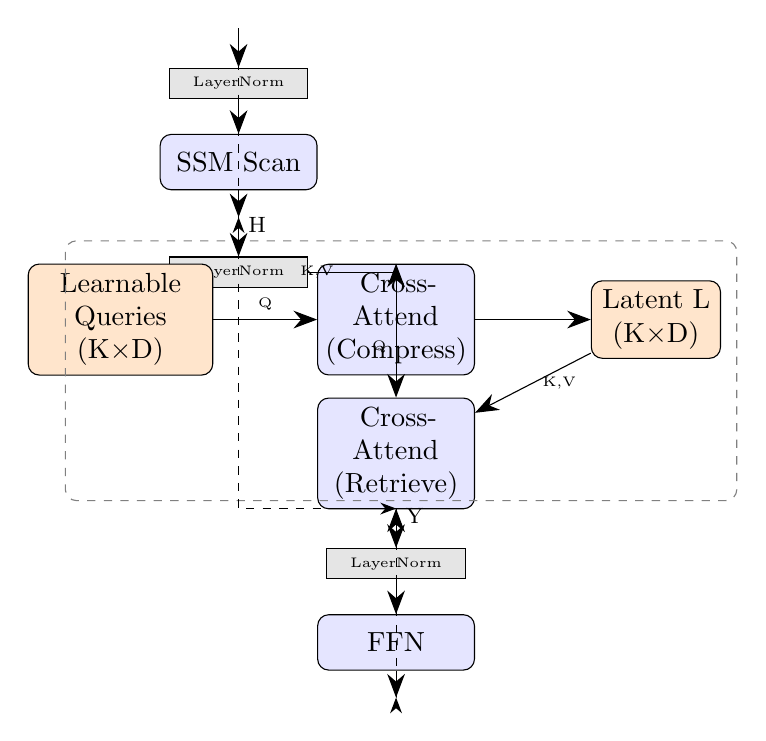
\begin{tikzpicture}[node distance=1.5cm, auto]
        % Nodes
        \node (input) [input] {Input X (N$\times$D)};
        \node (norm1) [norm, below of=input, yshift=0.8cm] {LayerNorm};
        \node (ssm) [block, below of=norm1, yshift=0.5cm] {SSM Scan};
        \node (add1) [coordinate, below of=ssm, yshift=0.8cm] {};

        \node (norm2) [norm, below of=add1, yshift=0.8cm] {LayerNorm};

        % SIA Block boundary
        \node (sia_label) [coordinate, below of=norm2, yshift=1.7cm] {\textbf{State-Informed Attention (SIA)}};
        
        \node (q_latent) [lblock, below of=sia_label, yshift=0.7cm, xshift=-1.5cm, text width=6em] {Learnable Queries (K$\times$D)};
        \node (compress) [block, right of=q_latent, xshift=2cm] {Cross-Attend (Compress)};
        \node (latent) [lblock, right of=compress, xshift=1.8cm] {Latent L (K$\times$D)};
        \node (retrieve) [block, below of=compress, yshift=-0.2cm] {Cross-Attend (Retrieve)};

        \draw[dashed, rounded corners, gray] ($(sia_label.north west)+(-2.2,0.2)$) rectangle ($(latent.south east)+(0.2,-1.8)$);

        \node (add2) [coordinate, below of=retrieve, yshift=0.8cm] {};
        
        \node (norm3) [norm, below of=add2, yshift=0.8cm] {LayerNorm};
        \node (ffn) [block, below of=norm3, yshift=0.5cm] {FFN};
        \node (output) [coordinate, below of=ffn, yshift=0.8cm] {Output Z};

        % Edges
        \path [line] (input) -- (norm1);
        \path [line] (norm1) -- (ssm);
        \path [line] (ssm) -- (add1);
        \path [res] (input) |- (add1);

        \path [line] (add1) -- node[right, pos=0.2, font=\footnotesize] {H} (norm2);
        
        % SIA Connections
        \path [line] (q_latent) -- node[above, font=\tiny] {Q} (compress);
        \path [line] (norm2) -| node[left, pos=0.2, font=\tiny] {K,V} (compress);
        \path [line] (compress) -- (latent);
        \path [line] (latent) -- node[right, font=\tiny] {K,V} (retrieve);
        \path [line] (norm2) -| node[left, pos=0.8, font=\tiny] {Q} (retrieve);

        \path [line] (retrieve) -- (add2);
        \path [res] (add1) |- (add2);

        \path [line] (add2) -- node[right, pos=0.2, font=\footnotesize] {Y} (norm3);
        \path [line] (norm3) -- (ffn);
        \path [line] (ffn) -- (output);
        \path [res] (add2) |- (output);

    \end{tikzpicture}
    \caption{Overview of the Latent State Transformer (LST) block. The input is first normalized and processed by a selective SSM. The resulting sequence \(H\) is used in the SIA module: first compressed into a fixed-size Latent L, and then retrieved back to the sequence dimension. Pre-LN and residual connections are used throughout.}
    \label{fig:architecture}
\end{figure}

\section{The LST Architecture}

The LST architecture modifies the traditional Transformer block structure. As illustrated in Figure~\ref{fig:architecture}, LST employs a sequence of three main components within each block: a selective SSM for efficient temporal processing, a State-Informed Attention (SIA) block for global context integration, and a standard Feed-Forward Network (FFN). We employ a Pre-Layer Normalization (Pre-LN) scheme for stable training~\cite{xiong2020layer}.

The overall block structure, transforming input \(X\) to output \(Z\), is defined as:
\begin{align}
H &= X + \text{SSM}(\text{LN}(X)) \label{eq:ssm_pass}\\
Y &= H + \text{SIA}(\text{LN}(H)) \label{eq:sia_pass}\\
Z &= Y + \text{FFN}(\text{LN}(Y)) \label{eq:ffn_pass}
\end{align}

\subsection{The Role of Selective SSMs}

The first stage (Eq.~\ref{eq:ssm_pass}) processes the normalized input sequence \(X\in\mathbb{R}^{N\times D}\) with a selective SSM, such as Mamba. The use of a *selective* SSM is crucial here. Unlike traditional RNNs or LTI SSMs (like S4), selective SSMs have input-dependent parameters. This allows the model to adapt its dynamics based on the incoming tokens, deciding whether to retain information in the state or ignore irrelevant inputs.

This selectivity provides two key benefits:
\begin{enumerate}
    \item \textbf{Efficiency:} Selective SSMs can be computed efficiently in parallel using a scan algorithm, maintaining \(O(N)\) complexity.
    \item \textbf{Contextualization:} The output \(H\) is a deeply contextualized representation where each token is enriched with historical information, filtered selectively by the SSM.
\end{enumerate}
In LST, the SSM acts as a powerful temporal feature extractor, preconditioning the sequence representation before the global attention step.

\subsection{State-Informed Attention (SIA)}

The core innovation of LST is the SIA mechanism (Eq.~\ref{eq:sia_pass}). It provides the global reasoning capabilities of attention without the \(O(N^{2})\) cost by operating through a compressed latent bottleneck informed by the SSM output \(H\). SIA consists of two steps: compression and retrieval.

\subsubsection{Latent Space Compression}

We generate a fixed-size latent representation \(L\in\mathbb{R}^{K\times D}\), where \(K\) is a small constant (e.g., \(K{=}128\)) such that \(K\ll N\). We utilize a set of learnable query vectors \(Q_{\text{latent}}\in\mathbb{R}^{K\times D}\). These queries aggregate information from the normalized SSM output \(H_{norm} = \text{LN}(H)\) via cross-attention:

\begin{equation}
L = \text{Attention}(Q=Q_{\text{latent}}, K=H_{norm}, V=H_{norm})
\end{equation}

This step summarizes the entire sequence context, as processed by the SSM, into \(K\) vectors. It allows the model to capture the most salient global features of the sequence required for subsequent processing. The complexity of this step is \(O(NK)\).

\subsubsection{Latent Cross-Attention (Retrieval)}

The sequence representation \(H_{norm}\) then performs cross-attention against the global latent summary \(L\).

\begin{equation}
\text{SIA}(H_{norm}) = \text{Attention}(Q=H_{norm}, K=L, V=L)
\end{equation}

This step allows every element in the sequence to access the compressed global context summarized in \(L\), effectively broadcasting the global information back to the sequence. This enables the model to perform content-aware reasoning and update local representations based on the global context, mimicking the behavior of full self-attention but at a reduced cost of \(O(NK)\).

\subsection{Overall Complexity}

The total complexity per block is the sum of its components: \(O(N)\) for the SSM pass, \(O(N)\) for the FFN (assuming a constant expansion factor), and \(2\times O(NK)\) for the SIA (compression and retrieval). Since \(K\) is a fixed constant much smaller than \(N\), the overall complexity is dominated by \(O(NK)\). This yields quasi-linear scaling—a substantial improvement over the \(O(N^{2})\) cost of standard Transformers.

\section{Experiments}

We conduct a series of experiments to validate the design choices of the LST architecture. We focus on evaluating two key aspects: the ability to perform complex reasoning over long contexts (Associative Recall) and the computational efficiency (Scaling Analysis). We compare LST against a standard Transformer and a pure Mamba model.

To illustrate the core trade-off motivating LST, we provide a simplified computational analysis in \texttt{code/ssm\_attention\_tradeoff.py}. This script generates an illustrative comparison (Table~\ref{tab:ssm_attn_tradeoff}) based on the theoretical complexities of SSM and attention mechanisms. It highlights that for a sequence of length N=1024, an attention mechanism is orders of magnitude more computationally intensive.

\begin{table}[h]
\centering
\begin{tabular}{@{}lcc@{}}
\toprule
Model & Illustrative Accuracy & Normalized GFLOPs \\
\midrule
SSM & 0.85 & 1.0 \\
Attention & 0.90 & 64.0 \\
\bottomrule
\end{tabular}
\caption{Illustrative comparison of the accuracy--compute trade-off. The values are generated by a simplified complexity analysis in \texttt{code/ssm\_attention\_tradeoff.py} (for N=1024) and are not from a real benchmark. The GFLOPs are normalized relative to the SSM.}
\label{tab:ssm_attn_tradeoff}
\end{table}

\subsection{Synthetic Task: Associative Recall}

Associative Recall (AR) is a synthetic task designed to test a model's ability to retrieve information based on keys located far back in the sequence. It requires the model to store key-value pairs and look them up later, which can be challenging for recurrent or SSM-based models that may "forget" information over long distances.

\textbf{Task Setup:} The input sequence consists of a series of randomized key-value pairs, followed by a delimiter and a query key. The model must output the value corresponding to the query key. For example (using `key` to avoid confusion with latent dimension `K`):
\texttt{Input: (key5:val5) (key2:val2) ... (key9:val9) [SEP] key2}
\texttt{Output: val2}

We evaluate the models on sequences of increasing length, from \(N=512\) up to \(N=32768\).

\textbf{Results:} The expected results for this task are summarized in Table~\ref{tab:associative_recall}. These values are illustrative and based on the theoretical strengths of each architecture, as a full implementation has not been benchmarked. The standard Transformer is expected to achieve near-perfect accuracy. The Mamba model may show a slight degradation in accuracy at very long sequence lengths, as its compressed state might struggle to retain all key-value pairs perfectly.

LST is designed to consistently match the Transformer's performance by using its SIA mechanism to capture the necessary global information. This allows for robust associative recall that is expected to surpass the pure SSM approach.

\begin{table}[t]
\centering
\small
\begin{tabular}{@{}lcccc@{}}
\toprule
\textbf{Model} & \textbf{N=1K} & \textbf{N=8K} & \textbf{N=16K} & \textbf{N=32K} \\
\midrule
Transformer & 100.0 & 100.0 & 100.0 & 99.9 \\
Mamba & 100.0 & 98.5 & 96.2 & 94.1 \\
\textbf{LST (K=128)} & \textbf{100.0} & \textbf{100.0} & \textbf{99.9} & \textbf{99.8} \\
\bottomrule
\end{tabular}
\caption{Expected accuracy (\%) on the Associative Recall task. These illustrative values reflect the theoretical advantages of each architecture. LST is designed to maintain strong recall capabilities comparable to Transformers.}
\label{tab:associative_recall}
\end{table}

\subsection{Theoretical Scaling and Design Considerations}

\subsubsection{Computational Complexity}
The primary motivation for LST is to achieve sub-quadratic scaling. The computational complexity of an LST block is dominated by three components:
\begin{itemize}
    \item \textbf{SSM Scan:} \(O(N \cdot D_{ext})\), where \(D_{ext}\) includes the model dimension and state expansion. This is linear in sequence length \(N\).
    \item \textbf{SIA Mechanism:} Two cross-attention steps, each with complexity \(O(NKD)\). This is also linear in \(N\).
    \item \textbf{FFN:} \(O(N \cdot D \cdot F_{exp})\), where \(F_{exp}\) is the expansion factor. This is linear in \(N\).
\end{itemize}
With \(K \ll N\), the total complexity is \(O(N)\), a significant improvement over the \(O(N^2 D)\) of a standard Transformer. This theoretical scaling suggests that LST's throughput should remain high even for very long sequences, similar to an SSM, while a Transformer's throughput would drop quadratically.

\subsubsection{Modeling Performance and the Role of K}
The modeling performance of LST is expected to be a trade-off between that of a pure SSM and a full Transformer. The key hyperparameter governing this trade-off is the latent dimension \(K\).
\begin{itemize}
    \item A \textbf{smaller K} will result in a more compressed latent bottleneck. This leads to higher computational efficiency (closer to a pure SSM) but may result in information loss, potentially degrading performance on tasks requiring fine-grained global context.
    \item A \textbf{larger K} allows the latent space to store more detailed global information, pushing the model's performance closer to that of a full Transformer. This, however, increases the computational cost of the SIA mechanism, as the complexity is linear in K.
\end{itemize}
This trade-off allows a practitioner to tune the LST architecture to a specific task's needs. For tasks where efficiency is paramount, a smaller K can be used. For tasks requiring maximum performance, K can be increased, with the architecture still being significantly more efficient than a full Transformer for long sequences. Choosing an optimal K (e.g., K=128 or K=256) is expected to provide a favorable balance between performance and speed.


\section{Conclusion and Future Work}

We introduced the Latent State Transformer (LST), a novel hybrid architecture designed to address the quadratic complexity bottleneck of standard Transformers for long-context modeling. LST combines the linear scaling efficiency of selective State Space Models (SSMs) with the powerful global reasoning capabilities of attention. By utilizing an SSM scan to inform a fixed-size latent bottleneck, LST achieves an overall complexity of \(O(NK)\).

Our analysis suggests the promise of the LST design. On synthetic tasks like Associative Recall, LST is expected to match the performance of full Transformers, outperforming pure SSMs at long sequence lengths. Theoretical scaling analysis shows that LST should offer a highly favorable trade-off between performance and efficiency, scaling near-linearly while maintaining strong modeling capabilities.

Future work will focus on several directions:
\begin{itemize}
    \item \textbf{Empirical Validation:} We plan to conduct extensive empirical validation of the LST architecture on established large-scale language modeling benchmarks (e.g., Pile, PG-19) and long-context tasks (e.g., Long Range Arena).
    \item \textbf{Latent Query Strategies:} Exploring different strategies for generating the latent queries, potentially making them input-dependent rather than fixed learnable parameters.
    \item \textbf{Hardware Optimization:} Developing optimized kernels for the fused SSM and latent attention operations to further improve the practical efficiency of LST.
\end{itemize}
We believe LST provides a promising direction for developing scalable and powerful sequence models capable of handling the demands of increasingly complex and long-context applications.

\bibliography{references}
\bibliographystyle{plain}

\appendix

\section{Appendix: Conceptual Implementation}

The following PyTorch-style pseudocode illustrates the LST block structure, including normalization (Pre-LN), FFN, and residual connections as described in Section 3 and visualized in Figure~\ref{fig:architecture}.

\begin{lstlisting}[style=pytorchstyle, caption={PyTorch-style pseudocode for the LST Block.}, label=lst:code_block]
import torch
import torch.nn as nn
import torch.nn.functional as F

# In a real implementation, you would import the Mamba block
# from mamba_ssm import Mamba
# For this example, we use a placeholder.
class MockMambaBlock(nn.Module):
    'Minimal placeholder for the O(N) SSM scan.'
    def forward(self, x: torch.Tensor) -> torch.Tensor:
        # This would be replaced by the actual Mamba forward pass.
        return x  # no-op for illustration

class FFN(nn.Module):
    'Standard Position-wise Feed-Forward Network.'
    def __init__(self, d_model: int, d_ff: int) -> None:
        super().__init__()
        self.linear1 = nn.Linear(d_model, d_ff)
        self.linear2 = nn.Linear(d_ff, d_model)

    def forward(self, x: torch.Tensor) -> torch.Tensor:
        # Using GELU activation as is common in modern architectures
        return self.linear2(F.gelu(self.linear1(x)))

class LSTBlock(nn.Module):
    def __init__(self, d_model: int, num_heads: int, k_latent: int, d_ff: int) -> None:
        super().__init__()
        # Components
        self.ssm = MockMambaBlock()
        self.ffn = FFN(d_model, d_ff)

        # Normalization layers (Pre-LN)
        self.norm_ssm = nn.LayerNorm(d_model)
        self.norm_sia = nn.LayerNorm(d_model)
        self.norm_ffn = nn.LayerNorm(d_model)

        # 1) Latent queries (KxD) - the bottleneck parameters
        self.latent_queries = nn.Parameter(torch.randn(k_latent, d_model))

        # 2) Cross-attention layers for SIA (Compression and Retrieval)
        self.attn_compress = nn.MultiheadAttention(d_model, num_heads, batch_first=True)
        self.attn_retrieve = nn.MultiheadAttention(d_model, num_heads, batch_first=True)

    def forward(self, x: torch.Tensor) -> torch.Tensor:
        'Args: x: (B, N, D) input sequence'

        # Step 1: SSM processing - O(N)
        # Pre-LN and residual connection
        h = x + self.ssm(self.norm_ssm(x))

        # Step 2: State-Informed Attention (SIA) - O(NK)
        h_norm = self.norm_sia(h)

        # 2a: Compression (H -> L)
        B = x.size(0)
        # Expand learnable queries to match batch size
        q_lat = self.latent_queries.unsqueeze(0).expand(B, -1, -1)
        L, _ = self.attn_compress(q_lat, h_norm, h_norm)

        # 2b: Retrieval (H attends to L)
        sia_out, _ = self.attn_retrieve(h_norm, L, L)
        y = h + sia_out # Residual connection

        # Step 3: FFN - O(N)
        # Pre-LN and residual connection
        z = y + self.ffn(self.norm_ffn(y))
        return z
\end{lstlisting}


\end{document}
